%!TEX root = report.tex
\exercise{Morphological operations}
Morphological operations is the technique of analyzing and processing images with operations based on set theory and topologies, among other things.
Using some basic operations such as erosion, dilation, opening and closing images can be processed in a robust and efficient manner, and allow for creation of more complex morphological operations.

\subsection{Dilation}
The goal is to write a function that implements dilation.
In terms of set theory the operation can be described as \(A \oplus B = \underset{b \in B}\bigcup A_b\).
This operation can be understood as the creation of the set of all the points that are in \(B\) when the center of \(B\) is contained in \(A\) as \(B\) moves inside \(A\).

This notion is at the basis of our implementation of the dilation function \texttt{IPdilate}.
It can dilate binary (logical) images with a 3 \(\times\) 3 structuring element with its origin at \((0, 0)\).
By default the so-called `cross element' is used.

Because \(A\) may grow larger the image must be padded during computation.
We have implemented the function \texttt{IPdilate} in the following way:
\matlabexternal{../IPdilate.m}
\subsection{Erosion}
Another basic operation of morphological image processing is erosion.
Erosion can be described in terms of set theory as the following set: \(A \ominus B = \underset{b \in B}\bigcap A_{-b}\).
This can also be interpreted as all the points from \(A\) where \(B\) `fits' in its entirety.
This means that a pixel \(p_0\) in \(A\) is only retained if all of is contained in \(A\), with \(B\)'s origin at \(p_0\).

Because \(A\) can never grow larger when eroded, padding of the image is not necessary as opposed to during dilation.
However, the original image needs to be padded because the overlay of the structuring element may fall out of range with the image.
We have implemented \texttt{IPerode} in the following function:
\matlabexternal{../IPerode.m}
\clearpage
\subsection{Testing}
We have also tested our implementations of the algorithms with binary images.
In this case, the algorithms were tested on the \texttt{wirebondmask} image, which can be seen in Figure~\ref{fig:original_wirebond}.
The results of the erosion and dilation are visible in Figures~\ref{fig:erosion} and~\ref{fig:dilation}, respectively.

\begin{figure}[htb]
 \centering
 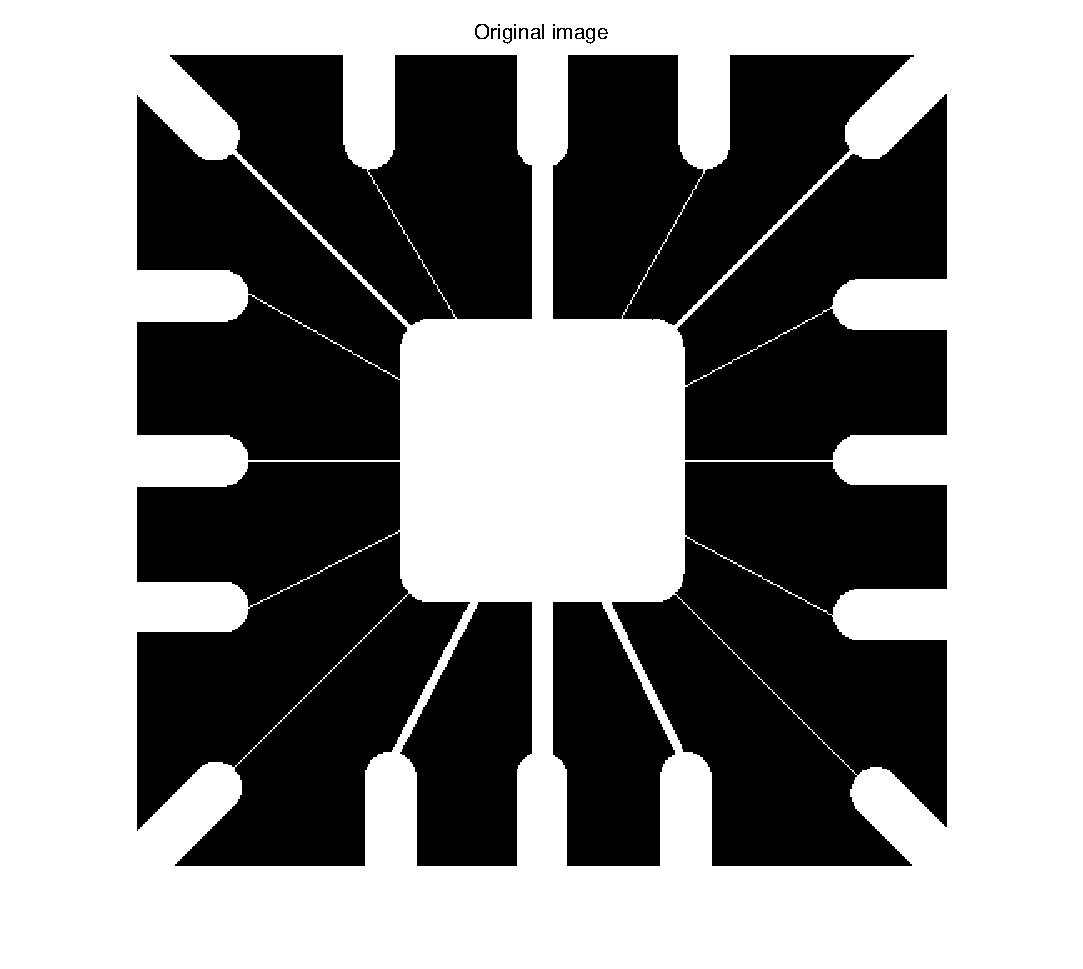
\includegraphics[width=\linewidth]{original_wirebond.eps}
 \caption{The original image}
 \label{fig:original_wirebond}
\end{figure}

\begin{figure}[htb]
 \centering
 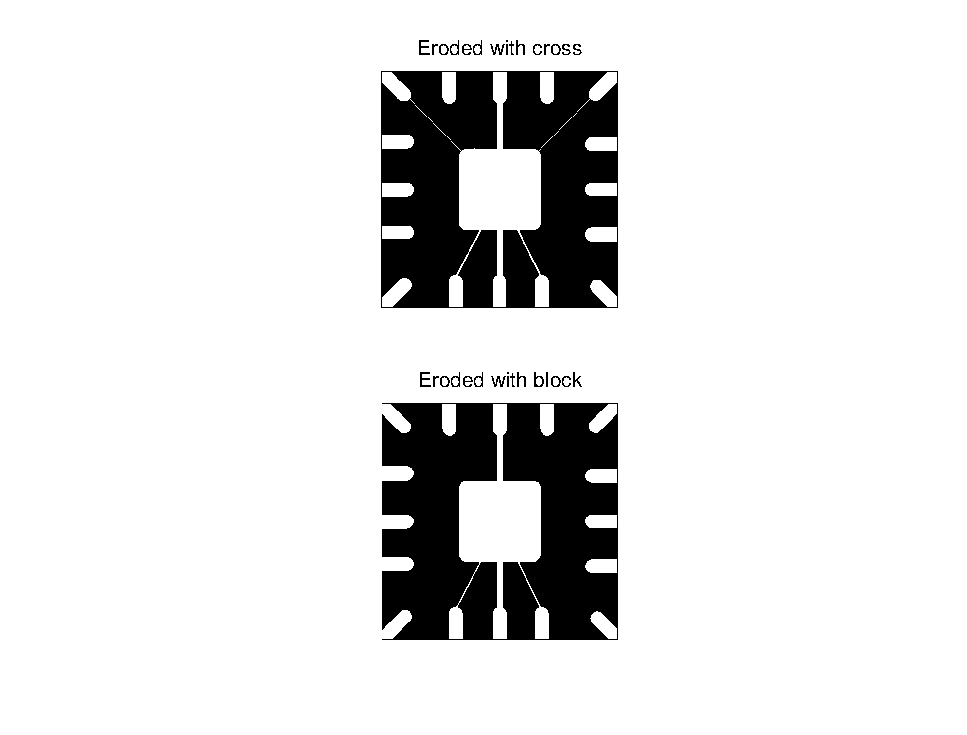
\includegraphics[width=\linewidth]{erosion.eps}
 \caption{Testing of our erosion function with several structuring elements}
 \label{fig:erosion}
\end{figure}

\begin{figure}[htb]
 \centering
 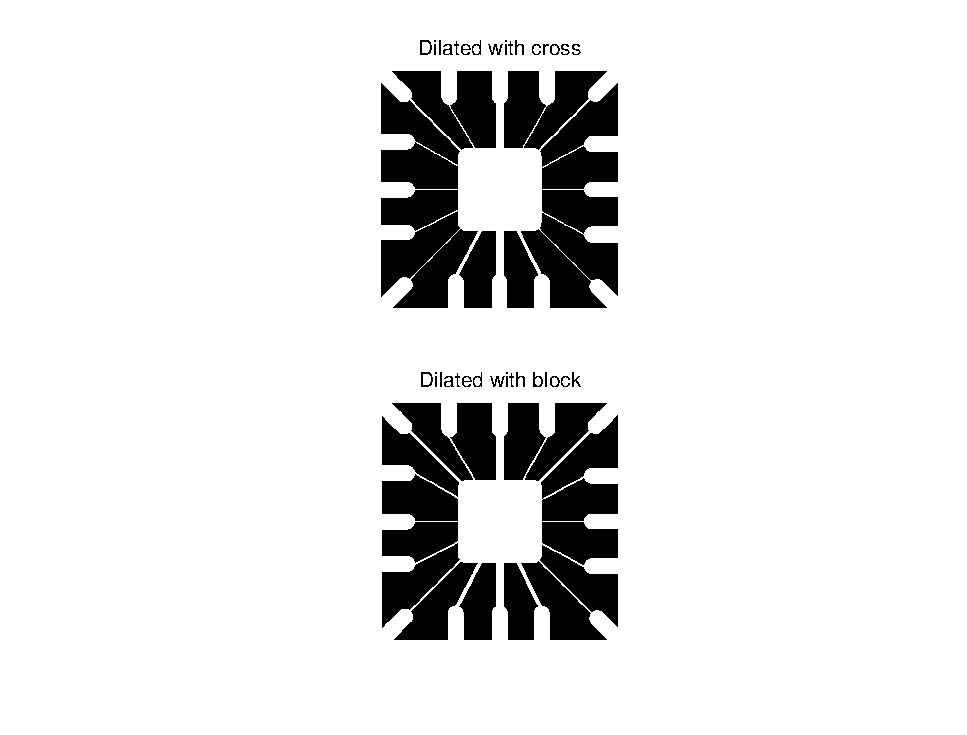
\includegraphics[width=\linewidth]{dilation.eps}
 \caption{Testing of our dilation function with several structuring elements}
 \label{fig:dilation}
\end{figure}

The difference between erosion and dilation are clear when comparing Figures~\ref{fig:erosion} and~\ref{fig:dilation}.
The effects are best visible at the `wires' running from the core of the image to the outer regions.
In the case of the dilation, the image grew larger thus the wires grew thicker.
In the case of erosion, the image grew smaller thus removing some lines entirely.

We have tested the algorithms for two different structuring elements.
Two of the dilations and erosions are computed using the cross element, \(\left(\begin{matrix}0 & 1 & 0 \\ 1 & 1 & 1 \\ 0 & 1 & 0 \end{matrix}\right)\), and the other two erosions and dilations are computed using the block element, \(\left(\begin{matrix}1 & 1 & 1 \\ 1 & 1 & 1 \\ 1& 1 & 1 \end{matrix}\right)\).
In the dilation case the results are not quite obvious, but more so in the erosion case.
It is very noticeable that different structuring elements deleted different wires of the image. 
Namely, the cross fits in the diagonal wires, whereas the block did not.

\clearpage